\documentclass[leqno,10pt]{article}

\usepackage{pgfplots}
% DO DRUKARNI i DO ILUSTROWANIA
\usepackage[hoffset={.2cm},voffset={1.7cm},papersize={216mm,301mm}]{geometry}
% DO ILUSTROWANIA
%\usepackage[hoffset={.2cm},voffset={1.7cm},papersize={210mm,297mm}]{geometry}

 \usepackage{tikz-3dplot}
\usepackage{circuitikz}
\usepackage{delta}
\usepackage{mathrsfs} 
\usepackage{lmodern}
\usepackage{tkz-euclide}
\usepackage{overpic}
\usepackage{circuitikz}
\usetikzlibrary{arrows.meta}
\usetikzlibrary{svg.path}
\definecolorset{cmyk}{}{}{magenta,1,.1,0,.1}

\definecolorset{cmyk}{}{}{magenta, 0 1 0 0}
\usetikzlibrary{snakes}
\usetikzlibrary{calc,through}
\usetikzlibrary{arrows,hobby}
\graphicspath{{rys/},{stale/}}
\usetikzlibrary{graphs}
\usetikzlibrary{math}
\def\xxxtkzMarkAngle(#1,#2,#3){\tkzFindAngle(#1,#2,#3)\tkzGetAngle{angle#1#2#3};
 \tkzDrawArc[R with nodes](#2,.65)(#3,#1)
 \tkzDrawArc[R with nodes](#2,.7)(#3,#1)}


\def\xtkzMarkAngle(#1,#2,#3){\tkzFindAngle(#1,#2,#3)\tkzGetAngle{angle#1#2#3};
 \tkzDrawArc[R with nodes](#2,.5)(#3,#1)}


\usetikzlibrary{decorations.markings}
\pagestyle{empty}

\usetikzlibrary{arrows.meta}

\usetikzlibrary{decorations.pathmorphing,patterns}
\usetikzlibrary{shapes.arrows}
\usetikzlibrary{decorations.pathreplacing,calligraphy}

\usetikzlibrary{patterns.meta}

\begin{document}
\scriptsize
\hrule width5.3cm height.2cm



\noindent
\lower5pt\rlap{%\kern.25cm %
 % \includegraphics[width=3.5cm]{lf-t800}
 \includegraphics[width=4cm]{lf-r793}
}%
% \noindent\rlap{\vbox to0pt{\vss
\kern.2cm

\def\rysc{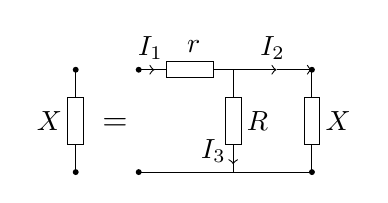
\begin{tikzpicture}
  \draw[fill=black](0,0) circle(.03) ;
  \draw[fill=black](0,1.3) circle(.03) ;
  \draw[fill=black](.8,0) circle(.03) ;
  \draw[fill=black](.8,1.3) circle(.03) ;
  \draw[fill=black](3,0) circle(.03) ;
  \draw[fill=black](3,1.3) circle(.03) ;
  \draw(0,0)--(0,1.3);
  \draw(3,0)--(3,1.3);
  \draw(2,0)--(2,1.3);
  \draw[->](.8,1.3)--(1,1.3);
 \draw[->](1,1.3)--(2.55,1.3);
  \draw[->](2.55,1.3)--(3,1.3);
  \draw[->](2,1.3)--(2,.1);
  \draw(.8,0)--(3,0);
  \draw[fill=white](1.15,1.2) rectangle(1.75,1.4);
  \draw[fill=white](-.1,.35) rectangle(.1,.95);
  \draw[fill=white](-.1+3,.35) rectangle(.1+3,.95);
  \draw[fill=white](-.1+2,.35) rectangle(.1+2,.95);
  \node[left] at(-.05,.65){$X$};
  \node[right] at(3.05,.65){$X$};
  \node[right] at(2.05,.65){$R$};
  \node at(.5,.6){\large$=$};
  \node[above] at (.95,1.3){$I_{1}$};
  \node[above] at (1.5,1.4){$r$};
  \node[above] at (2.5,1.3){$I_{2}$};
  \node[above] at (1.75,0){$I_{3}$};
\end{tikzpicture}}

\def\rysa{\begin{tikzpicture}
  \draw(0,0) rectangle(2,1.5);
  \draw(1,0) rectangle(3,2);
  \draw[white,fill=white](-.2,.65) rectangle(.2,.85);
  \draw(-.2,.65)--(.2,.65);
  \draw(-.2,.85)--(.2,.85);
  \draw[fill=white](.85,.6)--(1.15,.6)--(1,.9)--cycle;
  \draw(.85,.9)--(1.15,.9);
  \draw[fill=black](1,0) circle(.03) ;
  \draw[fill=black](1,1.5) circle(.03) ;
  \draw[white](2,.3) -- (2,1.2);
\draw [ snake=coil, segment amplitude=5pt, segment length=5pt]
(2,.3) -- (2,1.2);
\draw[white](3,.2)--(3,.6);
\draw[white](3,1.15)--(3,1.3);
\draw(2.9,1.15)--(3.1,1.15);
\draw(2.8,1.3)--(3.2,1.3);
  \draw[fill=black](3,.2) circle(.03) ;
  \draw[fill=black](3,.6) circle(.03) ;
  \draw(3,.6)--(3.2,.25);
  \node[below] at(3.3,.75){$K$};
  \node[below] at(1,0){$B$};
  \node[left] at(1.05,1.65){$B$};
\end{tikzpicture}}

\begin{tikzpicture}
  \draw(0,0) rectangle(3,3);
  \draw(-.1,.6)--(.1,.6);
  \draw[white](0,.6)--(0,.7);
  \draw(-.2,.7)--(.2,.7);
  \draw[fill=white](-.1,2.3) rectangle (.1,1.7) node[right,yshift=8]{$r$};
  \draw[white](.4,3) --(.8,3);
  \draw[fill=black](.4,3) circle(.04);
  \draw     (.8,3) -- +(140:.4);
  \draw[fill=black]     (.8,3) +(140:.4) circle(.04) ;
  \draw(1,0)--(1,3);
  \draw[fill=black](1,0) circle(.04) ;
  \draw[fill=black](1,3) circle(.04) ;
  \draw[fill=white](.85,2) rectangle (1.15,1) node[right,yshift=15]{$R$};
  \draw[white] (1.3,3) -- (2,3);
  \draw[white] (2.2,3) -- (2.9,3);
\draw [ snake=coil, segment amplitude=5pt, segment length=5pt]
  (1.3,3) -- (2,3)
  node [pos=0.5,below=.2] {$L_{1}$};
\draw [ snake=coil, segment amplitude=5pt, segment length=5pt]
  (2.2,3) -- (2.9,3)
  node [pos=0.5,below=.2] {$L_{2}$};
   \draw[fill=black](2.07,3) circle(.04) ;
   \draw(2.07,3)--(2.07,3.4)--(.8,3.4);
   \draw[fill=black](.8,3.4) circle(.04) ;
   \node at(.25,.5){$\mathcal E$};
   \node[above] at(.25,3){1};
  \node[above] at (.8,3.4){2};
     \end{tikzpicture}
\begin{tikzpicture}
    \def\cA{\begin{tikzpicture}\draw[fill=white](0,0) circle(.13);
        \node at(0,0){A};
      \end{tikzpicture}}
    \def\cV{
\begin{tikzpicture}\draw[fill=white](0,0) circle(.13);
        \node at(0,-.02){V};
      \end{tikzpicture}}
    \draw(3.5,0)--(0,0)--(0,1.3)--(3.5,1.3);
    \draw(1.3,0)--(1.3,1.3);
    \node at(1.3,.65){\cV};
\draw[fill=black](1.3,0) circle(.03);
\draw[fill=black](1.3,1.3) circle(.03);
    \begin{scope}[xshift=25]
    \draw(1.3,0)--(1.3,1.3);
    \node at(1.3,.65){\cV};
\draw[fill=black](1.3,1.3) circle(.03);
\draw[fill=black](1.3,0) circle(.03);
  \end{scope}
  \node at(.65,1.3){\cA};
  \node at(1.75,1.3){\cA};
  \node at(2.65,1.3){\cA};
\draw[fill=black](3.6,0) circle(.03);
\draw[fill=black](3.7,0) circle(.03);
\draw[fill=black](3.8,0) circle(.03);
\draw[fill=black](3.6,1.3) circle(.03);
\draw[fill=black](3.7,1.3) circle(.03);
\draw[fill=black](3.8,1.3) circle(.03);
\draw[white](0,.63)--(0,.7);
\draw[thick](-.15,.7)--(.15,.7);
\draw[thick](-.1,.63)--(.1,.63);
\end{tikzpicture}

\end{document}